% Timeline of concurrent work: batch chunks, a single request, DB pool, UI reads (Section 3.2).
\documentclass[tikz,border=1pt]{standalone}
% =====================================================================
%  Shared style for every diagram in the proposal.
%  Each figure is a standalone TikZ file that \input's this preamble, so
%  all diagrams use the same font family (Computer Modern, T1 -- identical
%  to the LLNCS body text), the same sizes and the same palette.
%
%  Font rule (do not change per figure):
%    node text   \footnotesize  (8 pt)
%    edge labels \scriptsize    (7 pt)
%    titles      \footnotesize\bfseries
%  Figures are drawn at their final width (<= 12.2 cm, the LLNCS text
%  width) and included WITHOUT scaling, so the printed size is the same
%  in every figure.
% =====================================================================
\usepackage[T1]{fontenc}
\usepackage{amsmath,amssymb}
\usepackage{xcolor}
\usepackage{tikz}
\usetikzlibrary{positioning,arrows.meta,shapes.geometric,shapes.multipart,
  fit,backgrounds,calc,shadows,patterns}

% ---- palette ---------------------------------------------------------
\definecolor{cBlue}{HTML}{0B4F8A}    % application / API
\definecolor{cOrange}{HTML}{B4540A}  % processing / services
\definecolor{cPurple}{HTML}{5B3CC4}  % data stores
\definecolor{cGreen}{HTML}{1B7A3A}   % success / output
\definecolor{cRed}{HTML}{B42318}     % error / risk
\definecolor{cGray}{HTML}{5F6672}    % external / neutral
\definecolor{cInk}{HTML}{1F2933}     % text and arrows

\colorlet{fBlue}{cBlue!9}
\colorlet{fOrange}{cOrange!10}
\colorlet{fPurple}{cPurple!9}
\colorlet{fGreen}{cGreen!10}
\colorlet{fRed}{cRed!9}
\colorlet{fGray}{cGray!8}

% ---- fonts -----------------------------------------------------------
\newcommand{\figfont}{\footnotesize}
\newcommand{\lblfont}{\scriptsize}
\newcommand{\code}[1]{\texttt{#1}}

\tikzset{
  every picture/.style={font=\figfont, line join=round, >={Stealth[length=4pt,width=3.4pt]}},
  every node/.append style={execute at begin node={\hyphenpenalty=10000\exhyphenpenalty=10000}},
  base/.style={draw, rounded corners=2pt, line width=0.6pt, align=center,
               inner xsep=3pt, inner ysep=2.5pt, text=cInk, font=\figfont},
  app/.style={base, draw=cBlue, fill=fBlue},
  svc/.style={base, draw=cOrange, fill=fOrange},
  data/.style={base, draw=cPurple, fill=fPurple},
  ok/.style={base, draw=cGreen, fill=fGreen},
  bad/.style={base, draw=cRed, fill=fRed},
  ext/.style={base, draw=cGray, fill=fGray},
  plain/.style={base, draw=none, fill=none},
  db/.style={cylinder, shape border rotate=90, aspect=0.22, draw=cPurple,
             fill=fPurple, line width=0.6pt, align=center, text=cInk,
             minimum height=9mm, font=\figfont},
  decision/.style={diamond, aspect=2.2, draw=cOrange, fill=fOrange,
                   line width=0.6pt, align=center, inner sep=1pt, text=cInk, font=\figfont},
  actor/.style={draw=cInk, fill=fGray, line width=0.8pt, rounded corners=0pt,
                align=center, inner sep=3pt, font=\figfont\bfseries},
  layer/.style={draw=cGray!60, fill=cGray!4, rounded corners=3pt, line width=0.5pt},
  layertitle/.style={font=\lblfont\bfseries, text=cGray, anchor=north west, inner sep=2pt},
  arr/.style={->, draw=cInk, line width=0.6pt},
  darr/.style={->, draw=cGray, line width=0.6pt, dashed},
  biarr/.style={<->, draw=cInk, line width=0.6pt},
  lbl/.style={font=\lblfont, text=cInk, inner sep=1.5pt},
  lblbg/.style={font=\lblfont, text=cInk, inner sep=1.5pt, fill=white},
}

% ---- UML sequence-diagram helpers -----------------------------------
%  \lifeline{id}{x}{label}{bottom y}   head box + dashed life line
%  \msg{x1}{x2}{y}{label}              synchronous call (solid)
%  \ret{x1}{x2}{y}{label}              reply (dashed)
%  \selfmsg{x}{y}{label}               call to self, label on the right
%  \fragment{kind}{guard}{x1}{y1}{x2}{y2}  combined fragment (alt/loop/par)
\newcommand{\lifeline}[4]{%
  \node[app, text width=19mm, minimum height=8.5mm, font=\figfont\bfseries] (#1) at (#2,0) {#3};
  \draw[cGray, dashed, line width=0.5pt] (#1.south) -- (#2,#4);}
\newcommand{\msg}[4]{%
  \draw[arr] (#1,#3) -- node[lbl, above] {#4} (#2,#3);}
\newcommand{\ret}[4]{%
  \draw[darr] (#1,#3) -- node[lbl, above] {#4} (#2,#3);}
\newcommand{\selfmsg}[3]{%
  \draw[arr] (#1,#2+0.12) -- ++(0.3,0) -- ++(0,-0.24) -- ++(-0.3,0);
  \node[lbl, anchor=west, align=left] at (#1+0.35,#2) {#3};}
\newcommand{\fragment}[6]{%
  \draw[cGray, line width=0.5pt] (#3,#4) rectangle (#5,#6);
  \node[anchor=north west, draw=cGray, fill=white, font=\lblfont\bfseries,
        inner sep=1.5pt, line width=0.5pt] at (#3,#4) {#1};
  \if\relax\detokenize{#2}\relax\else
  \node[anchor=north west, font=\lblfont, text=cGray, inner sep=1.5pt] at (#3+0.75,#4) {[#2]};\fi}
\newcommand{\activation}[3]{% x, y top, y bottom
  \draw[draw=cBlue, fill=fBlue, line width=0.5pt] (#1-0.07,#2) rectangle (#1+0.07,#3);}

\begin{document}
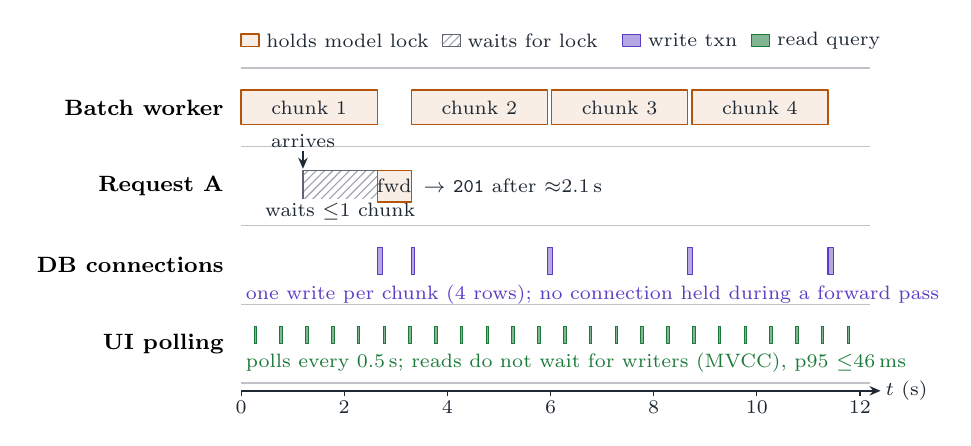
\begin{tikzpicture}[x=0.655cm, y=1cm]
  \def\L{0}   % lanes start (time 0)
  \tikzset{
    fwd/.style={draw=cOrange, fill=fOrange, line width=0.5pt},
    wr/.style={draw=cPurple, fill=cPurple!45, line width=0.4pt},
    rd/.style={draw=cGreen, fill=cGreen!55, line width=0.3pt},
    wait/.style={draw=cGray, pattern=north east lines, pattern color=cGray!60, line width=0.4pt},
    lane/.style={font=\figfont\bfseries, anchor=east, align=right},
  }
  % lanes
  \foreach \y/\t in {0/Batch worker, -1/Request A, -2/DB connections, -3/UI polling}{
    \node[lane] at (-0.15,\y) {\t};
    \draw[cGray!40, line width=0.4pt] (0,\y-0.5) -- (12.2,\y-0.5);
  }
  \draw[cGray!40, line width=0.4pt] (0,0.5) -- (12.2,0.5);
  % time axis
  \draw[arr] (0,-3.6) -- (12.4,-3.6) node[lbl, right] {$t$ (s)};
  \foreach \t in {0,2,...,12} \draw[cInk] (\t,-3.6) -- ++(0,-0.07) node[lbl, below] {\t};

  % batch worker: 4 tracks x 0.66 s = 2.64 s per chunk
  \foreach \a/\b/\n in {0/2.64/1, 3.30/5.94/2, 6.02/8.66/3, 8.74/11.38/4}{
    \draw[fwd] (\a,-0.22) rectangle (\b,0.22);
    \node[lbl] at ({(\a+\b)/2},0) {chunk \n};
  }
  % request A arrives at t = 1.2 s, waits for the lock, runs, writes
  \draw[cInk, line width=0.6pt, ->] (1.2,-0.55) -- (1.2,-0.78);
  \node[lbl, anchor=south] at (1.2,-0.57) {arrives};
  \draw[wait] (1.2,-1.2) rectangle (2.64,-0.8);
  \node[lblbg, fill=white] at (1.92,-1.32) {waits $\le$1 chunk};
  \draw[fwd] (2.64,-1.2) rectangle (3.30,-0.8);
  \node[lbl] at (2.97,-1.0) {fwd};
  \node[lbl, anchor=west] at (3.45,-1.0) {$\rightarrow$ \code{201} after $\approx$2.1\,s};

  % DB connections: borrowed only for short write transactions
  \foreach \a in {2.64, 5.94, 8.66, 11.38} \draw[wr] (\a,-2.12) rectangle (\a+0.1,-1.78);
  \draw[wr] (3.30,-2.12) rectangle (3.36,-1.78);
  \node[lbl, anchor=north west, text=cPurple] at (0,-2.2) {one write per chunk (4 rows); no connection held during a forward pass};

  % UI polling every 0.5 s, p95 20--46 ms
  \foreach \a in {0.25,0.75,...,11.75} \draw[rd] (\a,-3.0) rectangle (\a+0.05,-2.78);
  \node[lbl, anchor=north west, text=cGreen] at (0,-3.06) {polls every 0.5\,s; reads do not wait for writers (MVCC), p95 $\le$46\,ms};

  % legend
  \begin{scope}[shift={(0,0.85)}]
    \draw[fwd] (0,-0.08) rectangle (0.35,0.08); \node[lbl, anchor=west] at (0.4,0) {holds model lock};
    \draw[wait] (3.9,-0.08) rectangle (4.25,0.08); \node[lbl, anchor=west] at (4.3,0) {waits for lock};
    \draw[wr] (7.4,-0.08) rectangle (7.75,0.08); \node[lbl, anchor=west] at (7.8,0) {write txn};
    \draw[rd] (9.9,-0.08) rectangle (10.25,0.08); \node[lbl, anchor=west] at (10.3,0) {read query};
  \end{scope}
\end{tikzpicture}
\end{document}
